\documentclass[12pt]{report}
\usepackage{setspace}
\usepackage{here}
\usepackage{amsmath}
\usepackage[font=small,format=plain,labelfont=bf,up,textfont=up]{caption}
\usepackage[T1]{fontenc}
\usepackage{graphicx}
\usepackage{subfigure}
\usepackage{float}
\usepackage{listings}
\usepackage{courier}
\usepackage[ruled,vlined]{algorithm2e}
\usepackage{verbatim}

\author{Physically-based Rendering in Games}
\title{Guangfu Shi}

\begin{document}

\chapter{Introduction}

\chapter{BRDF}

\section{Radiometry Introduction}

\subsection{Important Quantities}

\begin{table}[ht]
\begin{center}
	
	\renewcommand{\arraystretch}{1.2}
	\begin{tabular}{ | l | l | l |}     	
	\hline

	Symbol & Quantity & Unit \\
	\cline{1-3}

	% \(Q_{\lambda}\) 	& 		Spectral radiant energy 		& 		\(J nm^{-1} \) \\
	\(Q\) 			& 		Radiant Energy 				& 		\(j\) \\
	\(\Phi\) 			& 		Radiant flux 					& 		\(W\) \\
	\(I\) 			& 		Radiant intensity 				& 		\(W sr^{-1}\) \\
	\(E\)			&		Irradiance (incident) 			&		\(W m^{-2}\) \\
	\(L\)			&		Radiance						&		\(W m^{-2} sr^{-1}\) \\
	
	\hline

	\end{tabular}
\end{center}
\caption{Important Radiometry Quantities}
\label{tab:radiometry_quantities}
\end{table} 

\section{BRDF} 

The \emph{Bidirectional Reflectance Distribution Function}, BRDF, is the mathematic tool describing the reflection of light encounters an surface. \(\omega_{i}\) is the incident lighting direction, \(\omega_{o}\) is the direction in which the reflected light leaving from the surface, and \(n\) is the normal vector at the location \(p\) on the surface. Given the incident radiance \(L_{i}(p, \omega_{i})\), we can find the outgoing radiance to the viewer, \(L_{o}(p, \omega_{o})\). 

The BRDF, \(f_{r}\), defines the relationship between differential reflected radiance and differential irradiance:
\begin{equation}
f_{r} = \frac{dL_{o}(p, \omega_{o})}{dE(p, \omega_{i})} = \frac{dL_{o}(p, \omega_{o})}{L_{i}(p, \omega_{i})(\omega_{i} \cdot n)d\omega{i}}
\label{eq:brdf}
\end{equation}

To compute the outgoing radiance given a surface normal, incident light direction and radiance and a BRDF, we have:
\begin{equation}
L_{o}(p, \omega_{o}) = \int_{\Omega}f_{r}(p, \omega_{i}, \omega_{o})L_{i}(p, \omega_{i})(\omega_{i} \cdot n)d\omega_{i}
\label{eq:local_render_equation}
\end{equation}

\section{Microfacet Reflection Model} 

\begin{figure}[htp]
    \centering
    \fbox{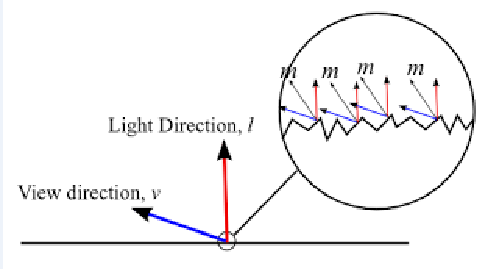
\includegraphics{figures/microfacet.pdf}}
    \renewcommand{\thefigure}{\thechapter.\arabic{figure}}
    \caption[Microfacet]{a surface is composed of many micro-facets and each micro-facet will only reflect light in a single direction according to their normal(m).}
    \label{fig:microfacet}
\end{figure}

So, in the above diagram, for light coming from direction \(l\) to be reflected to viewing direction \(v\), the micro-facet normal m must be equals to the half vector between \(l\) and \(v\).

A microfacet BRDF has the following form:
\begin{equation}
f_{microfacet}(l, v) = \frac{F(l, h)G(l, v, h)D(h)}{4(n \cdot l)(n \cdot v)}
\label{eq:microfacet_brdf}
\end{equation}

Where
\begin{itemize} 
\item{\(F\) is fesnel relectace term.}
\item{\(G\) is geometry term of shadowing masking between microfacet. }
\item{\(D(h)\) is normal distribution term describing how microfacet normals is distributed around direction half-vector \(h\)}
\item{\(l\) is the light direction. }
\item{\(v\) is the view direction. }
\item{\(n\) is the surface normal. } 
\item{\(h\) is the half vector between \(l\) and \(v\)} 
\end{itemize}

Two interpretations of BRDF: (1) Given a incident direction of a ray of light, the BRDF gives the relative distribution of reflected and scattered light over all outgoing directions. (2) Given a view direction, the BRDF gives the relative contribution of light from each incoming direction to the outgoing light. Both interpretations are illustrated in figure \ref{fig:brdf_interpretations}. 

\begin{figure}[htp]
    \centering
    \fbox{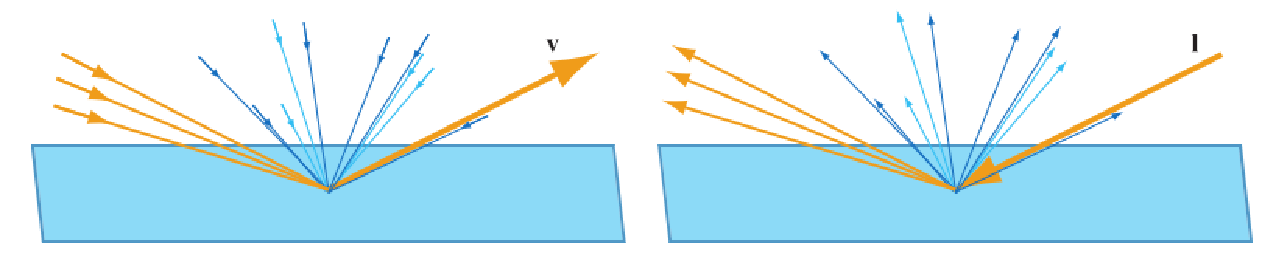
\includegraphics[width=\textwidth]{figures/brdf_interpretations.pdf}}
    \renewcommand{\thefigure}{\thechapter.\arabic{figure}}
    \caption[Microfacet]{Left side is (2), right side is (1).}
    \label{fig:brdf_interpretations}
\end{figure}


\subsection{Fresnel Term} 
A common used \emph{Schlick} approximation to the Fresnel equaiton is: 
\begin{equation}
F(f_{0}) = f_{0} + (1-f_{0})(1-l \cdot h)^{5}
\label{eq:schlick_fresnel}
\end{equation}

Where 
\begin{itemize}
\item{\(f_{0}\) is fresnel relectance term.}
\item{\(l\) is the incident light direction.}
\item{\(v\) is the view direction.} 
\item{\(h\) is the half vector between \(l\) and \(v\). } 
\end{itemize}

and \(f_{0}\) can be calculated by:
\begin{equation}
f_{0} = (\frac{1-n}{1+n})^2
\label{eq:fresnel_reflectance}
\end{equation}

\subsection{Distribution Term} 
Distribution term is used to describe how the microfacet normal distributed around a given direction (roughness). In the demo, I used two distribution function: Blinn-Phong and Beckmann distribution function.

\begin{equation}
D_{BlinnPhong}(h) = \frac{\alpha + 2}{2\pi}(n \cdot h)^{\alpha}
\label{eq:blinn_phong_distribution_term}
\end{equation}

\subsection{Geometry Term}
Geometry term is used for describing how much the microfacet is blocked by other microfacet. In games we usually use the implicit form: 

\begin{equation}
G_{implicit}(n, h, v, l) = (n \cdot l)(n \cdot v)
\label{eq:implicit_geo_term}
\end{equation}

\subsection{Rendering Equation in Games Rendering} 

Put all the terms above together, we have the microfacet specular BRDF, 
\begin{equation}
L_{o}(V) = \frac{\alpha + 2}{8}(n \cdot h)^{\alpha}F(f_{0},l,h)\otimes c_{light}(n \cdot l)
\label{eq:microfacet_spec_lo}
\end{equation}
where \(f_{0}\) is fresnel term that can be replaced with specular color \(c_{spec}\).


Add diffuse term, we have the final rendering equation:
\begin{equation}
L_{o}(V) = (c_{diff} + \frac{\alpha + 2}{8}(n \cdot h)^{\alpha}F(c_{spec},l,h)) \otimes c_{light}(n \cdot l)
\label{eq:microfacet_render_eq}
\end{equation}

\subsection{Energy between diffuse and specular reflection}







\end{document}

